\chapter{Background}
\label{ch:Introduction}
\section{General Introduction}
\label{sec:Science}
The race for the first quantum computer is on. Academic researchers and private
enterprises around the world are pursuing this goal, on a number of different
physical platforms. Here, I will describe my efforts towards achieving quantum
computation in linear optics.

Of course, building a full-scale, universal quantum computer is going to be
difficult, and beyond the scope of any single PhD student's research. At the
other end of the spectrum, some quantum technologies have already found
commercial viability, also putting them outside of the realms of academic
research. I will focus on the middle ground between these two extremes: quantum
computers that fall short of being universal for BQP, yet may be able to
outperform a classical computer at certain, specific tasks in the near future.

One such device would be the Boson Sampler. Proposed by Aaronson and Arkhipov
in~\cite{bosonsampling}, this is a device somewhat native to linear optics.
While it is
a good candidate for beating a classical computer, its uses are somewhat limited
at the moment. I will discuss two results relevant to building a Boson Sampler:
in chapter~\ref{ch:DirectDialling} I present a theoretical result concerning
Haar random unitary matrices; chapter~\ref{ch:QCV} presents a demonstration of
practical techniques to verify the output of such a device. Experimental results
presented in chapter~\ref{ch:QCV} could be said to be implementing
\bosonsampling{ }on a small scale.

The second class of quantum computer that I shall discuss is the quantum
simulator. The purpose of quantum simulation is to use a device that is well
understood and controlled, in order to simulate the behaviour of a quantum
system that is less accessible. In chapter~\ref{ch:Simulations} I present
experimental results of quantum simulations using linear optics. Two systems are
simulated: the (quantized) vibrations of molecules, and more abstract systems of
bosons obeying \(\pt\)-symmetric (but non-Hermitian) dynamics.

Once these devices begin to become larger, it is essential to have procedures to
test whether they are working correctly. Since the original point is to
outperform a classical computer, they cannot simply be checked by performing the
same calculations classically! Chapter~\ref{ch:QCV} presents methods for the
calibration, validation and verification of quantum devices. The calibration
procedure is described in detail for a circuit in bulk optics, which illustrates
many of the complicating features present in any large optical device. The
verification procedure is used to check the coherence \todo{how do I say this? I
mean indistinguishability of photons} of up to 5 photons in a quantum walk and 6
6 photons in a quantum Fourier transform.

Finally, chapter~\ref{ch:Hamiltomo} describes a tomography protocol that can be
used in certain circumstances to arrive at a complete description of the device
in question.

\section{Evolution of Quantum States}
\label{sec:Evolution}
The entire purpose of quantum mechanics is to calculate the evolution of quantum
systems. At any time, a system in a pure state can be completely described by
its wavefunction, \(\ket{\Psi}\) \cite{pbr}. In the non-relativistic
picture\footnote{I am restricting the discussion to non-relativistic quantum
mechanics, since it offers a valid description of the behaviour of photons,
perhaps surprisingly since they travel at the speed of light.} this
wavefunction evolves according to the Schr\"odinger equation, in terms of the
Hamiltonian, \(\op{H}\):
\begin{equation}
  \op{H} \ket{\Psi} = i \hbar \frac{\partial}{\partial t} \ket{\Psi}
\end{equation}
In the case of a Hamiltonian that is constant in time, we can integrate this
equation to obtain a time-evolution operator (sometimes referred to as a
propagator):
\begin{equation}
  \label{eq:expiht}
  \op{U} \of{t} = e^{-\frac{i}{\hbar} \op{H} t}
\end{equation}
This operator relates a known state of the system at time \(t_{0}\) to the state
of the system at a later (or earlier) time, \(t\), via
\begin{equation}
  \ket{ \Psi \of{t} } = \op{U} \of{t-t_{0}} \ket{ \Psi \of{t_{0}} }
\end{equation}
Another simple case to consider is when the Hamiltonian varies but is piecewise
constant in time. In this case each constant segment has its own time evolution
operator, \(\op{U}_{i}\) and  the overall time evolution operator is just the
(appropriately ordered) product of these:
\begin{equation}
  \op{U} = \op{U}_{n} \cdot \op{U}_{n-1} \dots \op{U}_{2} \cdot \op{U}_{1}
\end{equation}
When the Hamiltonian is Hermitian, which it must be for a closed quantum system
(in order to conserve energy), the time evolution operator is unitary.

In the case of photonics (or at least the cases that I will discuss in this
thesis), the state space is discrete and finite, meaning that the wavefunction
can be expressed exactly as a complex vector of unit magnitude. The number of
dimensions required is the number of optical modes, be they spatial,
polarisation or some other degree of freedom. The Hamiltonians that we consider
are piecewise constant in time (e.g. the application of a waveplate in bulk or
a directional coupler in integrated optics\footnote{between these optical
components, the Hamiltonian is diagonal with uniform elements.}) so the time
evolution operator is a natural description.

When considering Hamiltonians on a discrete (\(m\)-dimensional) space, for
example in the case of an \(m\) mode quantum walk \cite{walks-peruzzo}, the
matrix exponential in equation~\ref{eq:expiht} can be performed classically in
time polynomial in \(m\). This observation, along with the ability to realise
any unitary operator in linear optics (see section~\ref{sec:ReckScheme}), is the
basis of the quantum simulations performed in chapter~\ref{ch:Simulations}.

This model can be extended to consider non-Hermitian Hamiltonians, in which
case the same mathematics applies, but equation~\ref{eq:expiht} results in a 
non-unitary operator. Physically, we associate this with an open quantum system,
or a system coupled to some external degrees of freedom (an environment).
Chapter~\ref{ch:Simulations} also describes quantum simulations of this kind of
coupled system.

\section{A universal circuit for linear optics}
\label{sec:ReckScheme}
Any lossless\footnote{In practical devices, this approximation is very good.
\todo{1dB/cm in silica devices?}} linear optical device can be
described by a unitary matrix operating on the optical modes. A device with
\(m\) input and \(m\) output modes will be described by an \(m \by m\) unitary.
In~\cite{reck}, it is shown that the converse is true: any unitary matrix can
be realised by a linear optical circuit. A constructive proof of this is
presented, and a candidate `universal circuit' is proposed. Universal, in this
context refers to a linear optical circuit with adjustable components
(beamsplitters with variable reflectivity and variable phase shifts), which can
be configured into any unitary.

\begin{figure}
  \begin{subfigure}{\textwidth}
    \centering
    \includegraphics{figures/reck_original}
    \caption{The original Reck scheme, implemented in bulk optics. As with all
    circuits in bulk optics, achieving phase stability in this system would be
    very difficult.}
    \label{fig:ReckOriginal}
  \end{subfigure} \\
  \vspace{1cm} \\
  \begin{subfigure}{\textwidth}
    \centering
    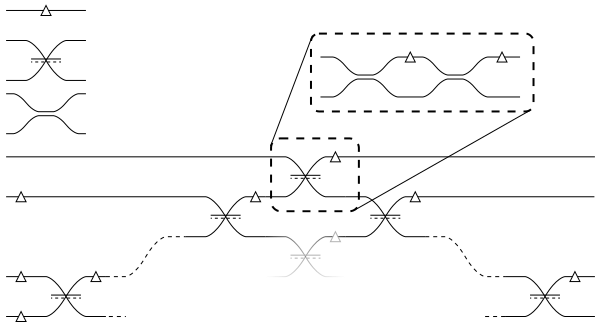
\includegraphics{figures/reck_general}
    \caption{A more modern take on the Reck scheme. Here we envisage using
    a triangular array of
    Mach-Zehnder interferometers (MZIs) on an integrated platform, thus solving
    the phase stability problem.}
    \label{fig:ReckGeneral}
  \end{subfigure}
  \caption[The Reck scheme, in both its original conception and an integrated
  optics version]{The Reck scheme, in both its original conception and an
  integrated
  optics version. In both systems, light enters from the left and the device
  performs a unitary transformation on the modes. Variable-reflectivity
  beamsplitters and variable phase shifts are needed in order to make the
  circuit's operation reconfigurable to any unitary transformation. In the
  bulk scheme, I have omitted any specifics, but in the integrated version these
  could be implemented with directional couplers and thermal or electro-optic
  phase shifts \todo{citation needed}.}
  \label{fig:ReckScheme}
\end{figure}

\section{Boson Sampling}
\label{sec:BosenSampling}
This section presents a review of \bosonsampling{}: a sampling algorithm
presented by Aaronson and Arkhipov in~\cite{bosonsampling}. None of development
or complexity analysis of this algorithm is my own work, but it provides useful
context for the material later in this chapter.

